\documentclass[german,12pt,a4paper]{article}
\usepackage{fullpage}
\usepackage[ngerman]{babel}
\usepackage[utf8]{inputenc}
\usepackage{listings}
\usepackage{verbatim}
\usepackage{enumerate}
\usepackage{graphicx}
\usepackage{float}
\usepackage{wrapfig}
\usepackage{color}
\usepackage[usenames,dvipsnames]{xcolor}
\usepackage[font=small,format=plain,labelfont=bf,up,textfont=it,up]{caption}
\usepackage{subfig}
\usepackage[colorlinks=false,pdfborder={0 0 0}]{hyperref}
\usepackage{eurosym}

\bibliographystyle{plain}
\pagestyle{plain}
\pagenumbering{arabic}
\frenchspacing

\newcommand{\comments}[1]{}
\renewcommand{\baselinestretch}{1.6}

%Redefine the first level
\renewcommand{\theenumi}{\textbf{\alph{enumi})}}
\renewcommand{\labelenumi}{\theenumi}

\begin{document}

\title{\textbf{SMS Versendung über Datenkanäle}}
\author{Sebastian Menski (734272), Martin Ohmann (734801) \\ \texttt{\{menski,ohmann\}@uni-potsdam.de}}
\date{\today}

\maketitle

\begin{abstract}
In dieser Arbeit geht es um die Gegenüberstellung des Short Message Service
GSM-Standards mit SMS-Alternativen, welche mobile Datennetze als Übertragungskanal
nutzen. Dazu wird die Funktionsweise von SMS über GSM und der Rich Communication Suite-enhanced
-- einer Realisierung über Datennetze -- beschrieben. Hierbei wird ein Überblick über die Nachteile
von SMS über GSM gegeben und Alternativen zur SMS aufgezeigt und gegenübergestellt. Abschließend
wird der aktuelle Zustand bewertet.
\end{abstract}

\section{Einleitung}

Durch die Einführung und Verbreitung des Mobilfunks und entsprechender Endgeräte hat sich neben der
Telefonie die Kommunikation über Textnachrichten als wichtiger Dienst herausgebildet. Die
geschichtliche Entwicklung dieser Dienste wird in Abschnitt \ref{sec:geschichte} beschrieben. Zur
Übermittlung von Textnachrichten wird im heutigen Mobilfunknetz vor allem durch der \textit{Short
Message Service (SMS)} genutzt. Dabei werden Textnachrichten über den \textit{Global System for
Mobile Communications (GSM)} Standard versendet und empfangen. Diese Nachrichten unterliegen
bestimmten Begrenzungen, diese und das Konzept der Übertragung werden in Abschnitt
\ref{sec:gsm} erläutert. Durch die Weiterentwicklungen im Bereich der Übertragungstechnik,
Mobilfunknetze und Endgeräte haben sich Alternativen zur klassischen SMS entwickelt. Diese und der
sogenannte \glqq{}Nachfolger der SMS\grqq{} werden in Abschnitt \ref{sec:datennetze} vorgestellt.
Zum Abschluss der Arbeit wird in Abschnitt \ref{sec:fazit} ein Fazit gegeben, welches den aktuelle
Zustand der mobilen Kommunikation bewertet.

\section{Geschichte}
\label{sec:geschichte}
Erste Überlegungen zu einem Textnachrichtendienst gab es bereits 1984 bei den 
europäischen Telekommunikationsgesellschaften. Damals wurde der ursprüngliche 
Konzeptvorschlag für den Short Message Service von Friedhelm Hillebrand von der 
damaligen Deutschen Bundespost mit Beiträgen von Bernard Ghillebaert von der PTT 
(Vorgänger der france Télécom) erarbeitet und schließlich 1985 in die 
GSM-Standarisierung eingebracht. Die erste Version des endgültigen Standards 
wurde 1989 verabschiedet. Finn Trosby von der norwegischen Telenor war es, der 
1987 bis 1990 als Leiter der Standardisierungsgruppe GSM4 DGMH (Drafting Group 
Message Handling) mit dieser das erste technische Design erarbeitete und 
standardisierte.
Vorn 1990 bis 2009 wurde der SMS-Standard in dieser Gruppe unter Leitung von 
Kevin Holly von Cellnet und Ian Harris von Vodafone weiterentwickelt\cite{wikipedia:sms}.

Die erste Kurzmitteilung des Short Message Service wurde am 3. Dezember 1992 
von einem PC an ein Mobiltelefon im britischen Vodafone-Netz gesendet. Dies 
war etwa ein Jahr nach der Einführung des GSM-Standards für Mobiltelefone in 
Europa.

\section{SMS über GSM} % {{{
\label{sec:gsm}

\subsection{Spezifikation}
SMS-Nachrichten werden durch das \textit{Short Message Service Center} (SMSC) des 
Providers verwaltet. Nachrichten werden vom Endgerät über Funk via dem 
Funkturm der Mobilfunkzelle an das SMSC gesendet und umgekehrt. Die 
Zugriffsprotokolle des SMSCs erlauben Interaktionen zwischen zwei SMSCs oder 
zwischen externen \textit{Short Message Entities} (SMEs) und einem SMSC. SMEs sind 
Software-Anwendungen auf Netzwerkkomponenten oder Hardware-Geräte, welche SMS
senden und empfangen können. Das \textit{Short Message Peer-to-Peer Protocol} (SMPP) 
wird hierbei für die Interaktion zwischen SMEs und SMSCs verschiedener 
Hersteller genutzt\cite{thesms}.

\begin{figure}[htm]
    \centering
	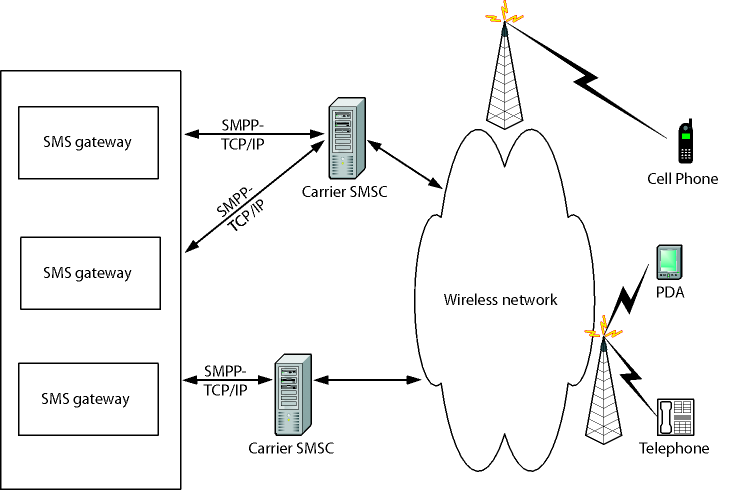
\includegraphics[width=0.9\textwidth]{img/smspp.png}
    \label{fig:smspp}
    \caption{Interaktionen zwischen SMSCs und SMEs}
\end{figure}	

Das SMSC arbeitet dabei entweder nach dem \textit{Store-and-Forward} oder 
\textit{Forward-and-Forget}-Prinzip. Beim \textit{Store-and-Forward}-Prinzip versucht das System 
die Nachricht regelmäßig für eine festgelegte Vorhaltezeit an den Empfänger 
zu übermitteln, bis diese erfolgreich bei ihm eingetroffen ist\cite{held:down}. Nachrichten, die innnerhalb 
der Vorhaltezeit nicht zugestellt werden konnten, werden von SMSC gelöscht. 
Ist die Empfängernummer dem SMSC unbekannt, lehnt es diese sofort an.
Arbeitet das SMSC nach dem \textit{Forward-and-Forget}-Prinzip, dann werden Nachrichten ohne 
Zwischenspeicherung an den Empfänger weitergeleitet. Es erfolgt hierbei keine Prüfung, 
ob die Nachricht auch tatsächlich angekommen ist. In der Regel wird von SMSCs überwiegend 
das \textit{Store-and-Forward}-Prinzip benutzt.

Eine SMS-Nachricht kann gewöhnlich bis zu 160 7-Bit-kodierte Zeichen beinhalten. 
Es sind jedoch auch 8-Bit- und 16-Bit-Kodierungen möglich. Hierbei beträgt die 
maximale Nachrichtenlänge 140 bzw. 70 Zeichen\cite{thesms}. 

SMS können auch dazu benutzt werden Binärdaten zu senden, wie zum Beispiel 
Klingeltöne oder Bildnachrichten. Spezielle Anwendungen auf 
dem Telefon übernehmen die Verarbeitung Dieser.


% \begin{figure}[h!]
%     \centering
%     \begin{tabular}{ p{4cm} | p{10cm} }
%         \textbf{Oktett(s)} & \textbf{Beschreibung} \\
%         \hline \hline
%          \texttt{07} & Länge der SMSC-Informationen (hier 7 Oktetts) \\ 
%          \hline
%          \texttt{91} & Typ der SMSC-Adresse (91 bedeutet internationales Telefonnummernformat) \\ 
%          \hline
%          \texttt{72 83 01 00 10 F5} & SMSC-Nummer (hier +27381000015) \\ 
%          \hline
%          \texttt{04} & Erstes Oktett dieser SMS-DELIVER message \\ 
%          \hline
%          \texttt{0B} & Länge der Adresse/Nummer des Senders (0B$_{16}$ = 11$_{10}$) \\ 
%          \hline
%          \texttt{C8} & Typ der Sender-Adresse \\ 
%          \hline
%          \texttt{72 38 88 09 00 F1} & Sender-Nummer (hier +27838890001) \\ 
%          \hline
%          \texttt{00} & Protocol identifier (00 = SME-to-SME Protokoll -- implizit) \\ 
%          \hline
%          \texttt{00} & Datenkodierung (00 = 7 bit, 01 = 8 bit, 10 = 16 bit, 11 = reserviert) \\ 
%          \hline
%          \texttt{99 30 92 51 61 95 80} & Zeitstempel \\ 
%          \hline
%          \texttt{0A} & Nutzdatenlänge/Länge der Nachricht \\ 
%          \hline
%          \texttt{E8 32 9B FD 46 97 D9 EC 37} & Nachricht "hellohello", 8-bit Oktetts representiert als 7-bit Daten
%     \end{tabular}
%     \label{tbl:sms-struct}
%     \centering
%     \caption{Beispiel der Transfer Protocol Data Unit: 
%         \texttt{07 91 72 83 01 00 10 F5 04 0B C8 72 38 88 09 00 F1 00 00 99 30 92 51 61 95 80 0A E8 32 9B FD 46 97 D9 EC 37}
%     }
% \end{figure}

\subsection{Nachrichtentypen}
Neben den normalen Kurznachrichten bietet der SMS-Standard noch drei weitere Textnachrichtentypen:
\begin{itemize}
	\item \textbf{Flash Message:} erscheint direkt auf Display des Empfängers. Die meisten Mobiltelefone 
        können solche Nachrichten nicht speichern. Ein Anwendungsbeispiel für solche Flash Messages ist die 
        Anzeige des Restguthabens direkt nach einem Gespräch.
	\item \textbf{Silent Message:} erscheinen weder auf dem Display noch durch akkustisches Signal. 
		Silent Messages werden z.B. von Polizei und Geheimdiensten zur Personenortung genutzt.
	\item \textbf{Concatenated Message:} Das System ist in der Lage überlange 
Nachrichten zu segmentieren. So werden bei Nachrichten, die länger als 160 Zeichen 
sind, mehrere SMS gesendet und später beim Empfänger wieder zusammengesetzt.
\end{itemize}

\subsection{Übertragung}
Zur Übertragung nutzt der Short Message Service nutzt einen Signalisierungskanel des GSM-Standards wie etwa SDCCH 
(\textit{Stand-alone Dedicated Control Channel}) oder FACCH (\textit{Fast Associated Control Channel}). 
Diese Kanäle werden auch genutzt, um Gespräche aufzubauen und zu halten.

Kurzmitteilungen können parallel zu Telefongesprächen empfangen/gesendet werden. Teil der Bandbreite des 
Verkehrsdatenkanals wird hier temporär zum Signailiserungskanal (SACCH) umkonfiguriert\cite{wikipedia:sms}.


\subsection{Technische Realisierung über GSM}
Der Short Message Service wird durch den \textit{Mobile Application Part} (MAP) des SS\#7 Protokolls (\textit{Signaling 
System No. 7}) realisiert\cite{3gpp:map}. Die Elemente des Short Message Protokolls werden als Felder innerhalb von 
MAP-Nachrichten durch das Netzwerk transportiert. Bei der Übertragung von Kurznachrichten vom Empfänger zum
Service Center wird die Prozedur \textit{Mobile Originated (MO) Short Message Service Transfer} genutzt,
für die Übertragung vom Service Center zum Empfänger die Prozedur \textit{Mobile Terminated (MT) Short
Message Service Transfer}. Zum Abhandeln von Fehlern und Verwalten von Warteschlangen stehen zudem die 
Prozeduren \textit{Short Message Alert} und \textit{Short Message Waiting Data Set} 
zur Verfügung\cite{3gpp:map}. Die Funktionsweise dieser Prozeduren wird im folgenden genauer beschrieben.


\subsubsection{Mobile Originated Short Message Service Transfer}
Immer wenn ein Nutzer eine SMS versendet, wird diese zum nächsten VMSC/SGSN (\textit{Mobile Switching 
Center/GPRS Core Network}) gesendet. Neben der Textnachricht werden Zieladresse und die Adresse des 
SMSCs übermittelt. 

Die Adresse des SMSCs ist hierbei in der Telefonkonfiguration der SIM-Karte definiert\cite{3gpp:smpp}. Das VMSC/SGSN 
ruft das MAP service package \textit{MAP\_MO\_FORWARD\_SHORT\_\-MESSAGE} auf um die Nachricht an das spezifizierte 
\textit{Interworking MSC} des Service Centers zu senden. Der Service sendet die \textit{mo-ForwardSM} MAP-Operation --
eingebettet in den \textit{Transaction Capabilities Application Part (TCAP)} -- an das SMSC, welches in der 
Nachricht angegeben wurde. Der Transport erfolgt hierbei über das \textit{Core Network} mittels des \textit{Signaling 
Connection Control Parts} (SCCP)\cite{3gpp:smpp}.

\begin{figure}[htm]
    \centering
	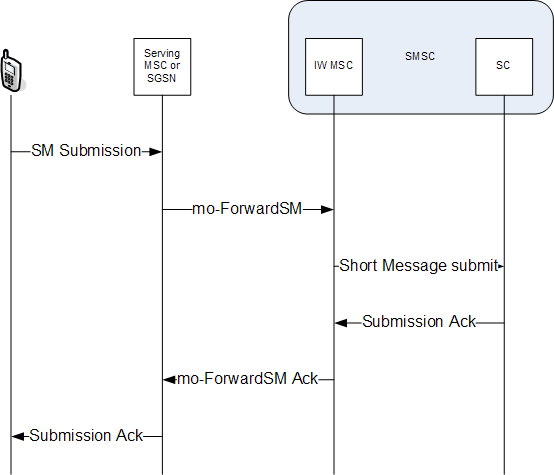
\includegraphics[width=0.9\textwidth]{img/mo-forward-sm.png}
    \label{fig:mo-forward-sm}
    \caption{Transport einer Kurznachricht vom Sender zum Service Center}
\end{figure}	

Nach Erhalt der \textit{mo-ForwardSM} MAP-Nachricht gibt das \textit{Interworking MSC} des SMSC die SMS-PP \textit{Application 
Protocol Data Unit} (APDU) (beinhaltet den Nachrichtentext) an das zuständige Service Center des SMSC 
weiter\cite{3gpp:techrel}. Hier wird sie gespeichert und anschließend versucht an die Zieladresse auszuliefern. Das 
Service Center liefert als Submission Status eine Erfolgs- oder Fehlermeldung zurück.

Nach Erhalt des Submission Status vom Service Center sendet das \textit{Interworking MSC} eine Benachrichtigung
zurück an das VMSC/SGSN des Senders. Von dort aus wird die Benachrichtigung über Funk an den Sender
ausgeliefert.


\subsubsection{Mobile Terminated Short Message Service Transfer}
Wenn das SMSC feststellt, dass es eine SMS ausliefern soll, dann sendet es die SMS-PP APDU der Nachricht 
an die \textit{Gateway MSC} (GMSC) Komponente des SMSC\cite{3gpp:techrel}. Das GMSC muss nach dem Empfangen der Nachricht die Position
des Empfängers herausfinden (in diesem Zusammenahng ist der Begriff \textit{Gateway MSC} ein \textit{Mobile Switching Center}, das Routing 
Informationen aus dem \textit{Home Location Register} (HLR) bezieht). Dies geschieht, indem das GMSC das MAP-Servicepaket 
\textit{MAP\_SEND\_ROUTING\_INFO\_FOR\_SM} aufruft, welches eine \textit{sendRoutingInfoForSM} (SRI-for-SM) 
MAP-Nachricht an das HLR der Zielnummer sendet, um die aktuelle Position des Empfängers anzufragen.
Die SRI-for-SM-Nachricht kann entweder an ein HLR im gleichen Netzwerk, oder aber über eine Verbindung zu
einem HLR in einem fremden PLMN (\textit{Public Land Mobile Network}) gesendet werden, je nachdem zu welchem 
Netzwerk der Empfänger gehört.

Das HLR führt eine Datenbanksuche durch und sendet die Daten zur aktuellen Position des Empfängers an das 
GMSC des SMSCs zurück. Diese Positionsdaten können entweder die Adresse des \textit{Mobile Switching Centers} sein, über welches der 
Empfänger gerade erreichbar ist, die SGSN Adresse, oder beides. Das HLR kann ebenfalls eine Fehlermeldung 
zurücksenden, fall der Empfänger nicht für Kurznachrichten geeignet ist.

Sobald das GMSC die Routing Informationen erhalten hat, versucht es die Nachricht an den Empfänger zu 
übermitteln. Diese geschieht die das Aufrufen des \textit{MAP\_MT\_\-FORWARD\_SHORT\_MESSAGE} Services, welcher eine
\textit{mt-ForwardSM} MAP-Nachricht an die vom HLR bereitgestellte Adresse sendet. Dabei ist es egal, ob es sich 
hierbei um ein MSC oder SGSN handelt.

Das VMSC fragt die benötigten Informationen zum Ausliefern der Nachricht beim \textit{Visitor Location Register}
(VLR) durch eine \textit{Send\_Infor\_for\_MS\_SMS} Nachricht ab. Das VLR sucht daraufhin nach dem Empfänger und
liefert die \textit{Mobile Subscriber ISDN Number} (MSISDN) des Empfängers an das VMSC zurück. Im Fehlerfall wird 
eine Benachrichtigung an das VMSC gesendet, die Auslieferung des SMS abgebrochen, und der gescheiterte 
Zustellversuch beim SMSC gemeldet. Em Erfolgsfall sendet das VMSC eine Erfolgsnachricht an das SMSC.

Die GMSC Komponente des SMSC reicht das Ergebnis des Zustellversuchs an das Service Center weiter. Im
Erfolgsfall wird die Nachricht aus der \textit{Store and Forward Engine} (SFE) entfernt und -- falls angefordert --
ein Zustellreport an den Sender geschickt\cite{3gpp:techrel}. Bei einem gescheiterten Zustellversuch versucht das SMSC
periodisch die Nachricht für eine bestimmte Vorhaltezeit zuzstellen. Das SMSC registiert sich eventuell 
beim HLR, um über eine erneute Verfügbarkeit des Empfängers benachrichtigt zu werden.

\begin{figure}[htm]
    \centering
	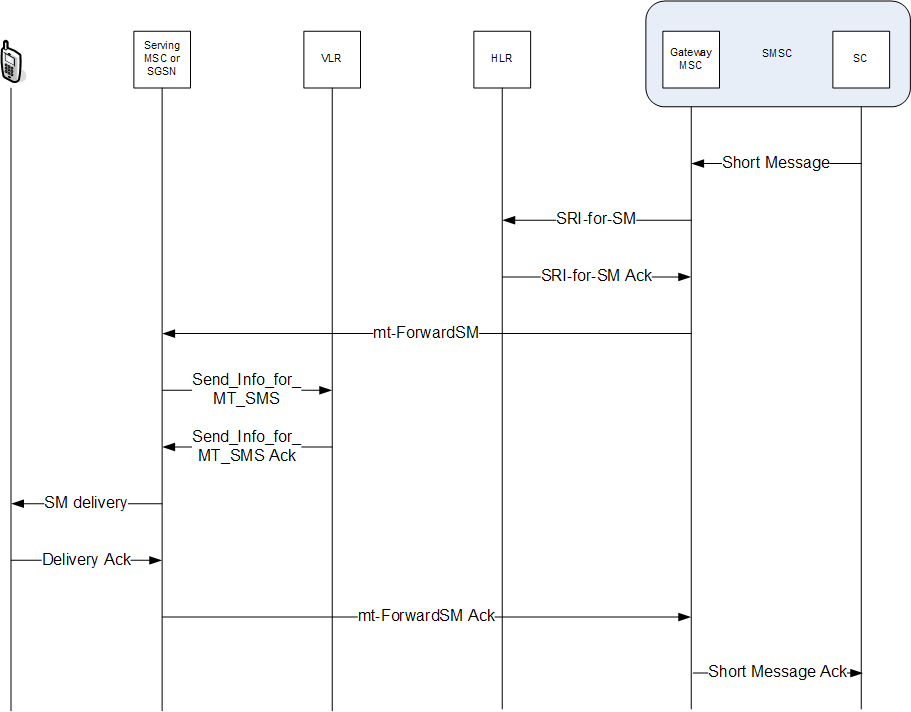
\includegraphics[width=0.9\textwidth]{img/mt-forward-sm.png}
    \label{fig:mt-forward-sm}
    \caption{Transport einer Kurznachricht vom Service Center zum Empfänger}
\end{figure}	

\subsubsection{Gescheiterte Zustellung und Warteschlange}
Falls das SMSC/SGSN einen Fehler bei der Auslieferung anzeigt, dann sendet das SMSC mit Hilfe der 
MAP-Prozedur \textit{MAP\_REPORT\_SM\_DELIVERY\_STATUS} eine Nachricht an das HLR, welche den Grund des Fehlers
angeibt und zusätzlich eine Anfrage zur automatischen Benachrichtigung des SMSC durch das HLR über die 
Zieladresse stellt.

Das HLR setzt ein Flag für den Zielaccount, welches angibt, dass dieser momentan für die Übermittlung von 
Kurznachrichten nicht verfügbar ist und speichert die Adresse des SMSCs in der \textit{Message Waiting Data} (MWD) 
Liste des Ziels. Gültige Flags sind hierbei: \textit{Mobile Not Reachable} (MNRF), \textit{Memory Capacity Exceeded} (MCEF) und
\textit{Mobile Not Reachable for GPRS} (MNRG). Ab diesem Zeitpunkt antwortet das HLR auf SRI-for-SM-Anfragen mit 
einem Fehler und fügt die Adressen der anfragenden SMSC automatisch der MWD-Liste des Ziel hinzu. Sollte 
eine SRI-for-SM-Anfrage ein gesetztes Priority Flag haben, dann antwortet das HLR mit der VLR-Adresse, 
falls diese verfügbar ist.

Das HR kann auf verschiedenen Wegen über die erneute Verfügbarkeit für Kurznachrichten eines Teilnehmers 
informiert werden:
\begin{itemize}
    \item Der Teilnehmer wurde vom Netzwerk getrennt. Eine Neuverbindung löst ein Location Update beim 
    HLR aus.
    \item Der Teilnehmer befand sich in einem ``Funkloch'', wurde jedoch nicht komplett vom Netzwerk
    getrennt. Beim erneuten Eintritt in einen abgedeckten Netzbereich antwortet es auf Page Requests
    des VLRs. Das VLR sendet daraufhin eine Ready-for-SM Nachricht and das HLR.
    \item Wenn der Telefonspeicher voll war und der Teilnehmer daraufhin einige Nachrichten löscht, so
    wird eine Ready-for-SM-Nachricht vom VMSC/VLR an das HLR gesendet.
\end{itemize}

Sobald das HLR über die erneute Verfügbarkeit des Teilnehmers informiert wurde, sendet es eine AlertSC 
MAP message an jedes in der MWD Liste des Teilnehmers registierte SMSC, wodurch der SMS-Zustellprozess
erneut gestartet wird\cite{3gpp:map}.

% \subsection{Message aggregators}
% \begin{itemize}
% 	\item Provider kommunizieren in der Regel nicht direkt mit SMSCs, sondern nutzen einen SMS Broker (oder message aggregator)
% 	\item Ein Aggregator ist eine Wirtschaftseinheit, welcher Verträge mit Netzwerk-Providern aushandelt und als Mittelsmann
% 		Zugang zu Mobilfunknetzen zur Nachrichtenübertragung für Dritte ohne direkte Beziehung zum Mobilfunknetzwerk gewährt. 
% 	\item Der Aggregator nutzt SMPP um Verbindungen mit Provider-Mobilfunknetzwerken aufrechtzuerhalten.
% 	\item Aggregatoren bieten Zugriff auf ihre Server typischerweise über SMPP oder kundenspezifische APIs an.
% 	\item \textit{Grafik SMSC, SMPP, SMS Broker anführen \\(Computer-SMS\_pdf.pdf, Figure 1)}
% \end{itemize}


\subsection{Nachteile von SMS über GSM}
Mit der voranschreitenden Entwicklung der mobilen Datennetze und Endgeräte ist die klassische SMS über GSM  in vielen Belangen
nicht mehr zeitgemäß und bietet eine ganze Reihe an Nachteilen:
\begin{itemize}
	\item \textbf{Multi-Device:} Der SMS Service ist an eine einzige Mobilfunknummer gebunden, was in der heutigen Zeit -- 
		wo Laptops, Tablets, Smartphones und PCs benutzt werden -- einen großen Nachteil gegenüber SMS Alternativen 
		bildet, welche die Möglichkeit bieten, einen Account auf mehreren Geräten gleichzeitig nutzen zu können.
	\item \textbf{Kosten:} SMS sind teuer. Ein Rechenbeispiel: Geht man von 16 Cents/SMS aus, dann entspricht das bei einer Länge von 
        140 Bytes pro Nachricht Kosten in Höhe von 0.11 Cents pro Byte. Bei einer Datenflat für \EUR{30} pro 2GB entspricht das 
        0.000003 Cents pro Byte. Die Kosten einer Datenflat sind also für den Nutzer wesentlich attraktiver als die Kosten für 
        herkömmliche SMS-Nachrichten.
	\item \textbf{Real-Time:} Es gibt keine Garantie für die Zustellzeit. Die Zustellung kann manchmal viel Zeit in Anspruch nehmen. 
		Desweiteren gibt es kein ``is typing'' Feature, welches aus vielen anderen Messengern bekannt ist. Apple iMessage z.B. bietet 
		dieses Feature und kommt zudem mit geringeren Zustellzeiten aus.
	\item \textbf{Gruppen:} Nachrichten an eine Gruppe von Personen sind in SMS nicht möglich. Es ist zwar möglich, eine Nachricht 
        an mehrere Personen gleichzeitig zu senden, jedoch sind diese voneinander unabhängig. Die Empfänger können nicht sehen, 
        an welche Personen die Nachricht ebenfalls gesendet wurde und haben somit keine Möglichkeit der Gruppe als Ganzes zu antworten.
	\item \textbf{Rich Text:} Die Limitation auf 160 7-Bit Zeichen lässt keine besonderen Formatierungen oder Schriftarten zu. 
        Das Einbetten von Grafiken, Emoticons und anderen Multimediainhalten ist nicht möglich. Enhanced Messaging Service Nachrichten 
        füllen diese Lücke.
	\item \textbf{Übertragungskanal:} Zur Übertragung wird der Signalisierungskanal des GSM-Standards verwendet. Ursprünglich waren 
        SMS-Nachrichten dazu gedacht, Mitteilungen über Netzstörungen oder ähnliche Informationen an den Nutzer zu senden. Dementsprechend 
        wurde der Übertragungskanal für das heutige Aufkommen an SMS-Nachrichten nicht ausgelegt.
\end{itemize}

In den letzten Jahren haben sich viele SMS-Alternativen entwickelt, welche den Nachrichtenversand über mobile Datennetze realisieren und 
nicht den Limitationen des GSM-Standards unterliegen.

% \subsection{SMS-Versand in Deutschland, Statistiken}
% \begin{itemize}
% 	\item SMS mittlerweile fast 20 Jahre alt (erste SMS überhaupt wurde am 3. Dezember 1992 verschickt)
% 	\item \textit{1999 - 2007, Grafik anfügen http://www.bitkom.org/de/presse/49919\_49417.aspx}
% 	\item \textit{2006 - 2011, Grafik anfügen http://www.bitkom.org/de/presse/64046\_67951.aspx}
% 	\item 2000: 11,4 Mrd. SMS
% 	\item 2005: \textgreater 22 Mrd. SMS
% 	\item 2010: \textgreater 41 Mrd. SMS, 1300 SMS pro Sekunde (78k/min)
% 	\item Stand 2011: 83\% aller Deutschen ab 14 Jahren besitzen ein Mobiltelefon: ca. 59Mio.
% \end{itemize}

% \subsection{MMS}
% \begin{itemize}
% 	\item nutzt Multimedia Messaging Service Center (MMSC)
% 	\item Übertragung über GPRS, Kommunikation mit Endgerät über WAP
% 	\item Spezifikation beinhaltet Schnittstellen zur Kommunikation mit E-Mail-Gateways und anderen MMSCs, die auf 
% 		SMTP beruhen; zur Komm. mit Value Added Services (VAS) wird SOAP verwendet
% 	\item Kodierung des Nachrichtenbodies basiert auf MIME
% 	\item MMS im Vergleich zu SMS viel stärker an E-Mail angelehnt
% \end{itemize}

% \section{Rich Communication Suite} % {{{
% \label{sec:rcs}

% \subsection{Übersicht} % {{{
% \label{sub:uebersicht}

% Quelle: \url{http://en.wikipedia.org/wiki/Rich\_Communication\_Suite}
% \begin{itemize}
% 	\item Industriestandard zur Nutzung des \textit{IP Multimedia Subsystem (IMS)} für Kommunikation von mobilen
% 		Endgeräten
% 	\item Für den Enduser: Sprachkommunikation, Instant Messaging, Videotelefonie,
% 		Kontakliste
% 	\item Main features: Enhanced Phonebook, Enhanced Messaging, Enriched Call
% 	\item Es werden verschiedene Standards genutzt, z.B. von \textit{3GPP} und  \textit{Open Mobile
% 		Alliance (OMA)} definiert, um das Enhanced Phonebook zu realisieren 
% 	\item RCS nutzt \textit{IMS} als Service-Platform zur Authentifizierungen, Autorisierung,
% 		Registration, Abrechnung und Routing
% 	\item Bestandteile des RCS-Konzepts:
% 		\begin{itemize}
% 			\item Präsenzinformation
% 				(\url{http://de.wikipedia.org/wiki/Pr%C3%A4senzinformation})
% 			\item Sprachtelefonie
% 			\item Instant Messaging
% 			\item Videoübertragung
% 			\item Bildübertragung
% 			\item SMS
% 			\item MMS
% 			\item Ortung
% 		\end{itemize}
% \end{itemize}

% % subsection uebersicht} }}}

% \subsection{Entwicklung} % {{{
% \label{sub:entwicklung}

% Quelle: \url{http://de.wikipedia.org/wiki/Joyn}
% \begin{itemize}
% 	\item Begann 2008 auf Initiative Nokias
% 	\item Wird vom Branchenverband \textit{GSM Association (GSMA)} vorrangetrieben
% 	\item Wird als \textit{Joyn} vermarktet und als "Nachfolger der SMS"
% 	\item Unterstützung von den Betriebssystemen Windows Mobile, iOS und Android
% 	\item Anfangs Einbindung durch Apps später im Betriebssystem verankert
% 	\item Offizielle Premiere auf der \textit{GSMA Mobile World Congress 2012 (MWC)}
% \end{itemize}

% % subsection entwicklung }}}

% \subsection{Einführung} % {{{
% \label{sub:einfuehrung}

% \begin{itemize}
% 	\item Vodafone Spanien startet Anfang 2012 eine \textit{Joyn} beta und bietet dazu eine Android App an
% 		(bis zum 13.01.2013 kostenlose Nutzung)
% 	\item In Deutschland:
% 		\begin{itemize}
% 			\item Vodafone Juni 2012 \url{http://www.vodafone.de/unternehmen/presse/pm-archiv-2012i_199573.html}
% 			\item T-Mobile Oktober 2012
% 			\item O2 2013
% 		\end{itemize}
% \end{itemize}

% subsection einfuehrung }}}

% section rcs }}}

\section{SMS über Datennetze} % {{{
\label{sec:datennetze}

 Durch die Erweiterungen \textit{General Packet Radio Service
(GPRS)} und \textit{Enhanced Data Rates for GSM Evolution (EDGE)} des GSM-Standards wurde die
paketvermittelte Datenübertragung möglich. Und mit den nachfolgenden Mobilfunkstandards
\textit{Universal Mobile Telecommunications System (UMTS)} und \textit{Long Term
    Evolution (LTE)} wurde die maximale Datenraten deutlich erhöht. Ein Vergleich der Datenraten
der verschiedenen Standards ist in Abbildung \ref{fig:datenraten} zu sehen. Die Möglichkeit
große Datenmenge schnell und effizient zu übertragen widerspricht dem Konzept der Standard-SMS
und ihren Beschränkungen. Daher wurde mit der GPRS Erweiterung auch der \textit{Multimedia
    Messaging Service (MMS)} eingeführt. Dieser ermöglicht es multimediale Nachrichten
mit wesentlich geringeren Beschränkungen als die klassische SMS zu versenden. Allerdings
konnte sich MMS nie wirklich durchsetzen. Gründe dafür könnten die hohen Preise der
Mobilfunkanbieter oder die teilweise komplizierte Konfiguration der Endgeräte sein. Daher
entwickelten sich alternative Lösungen von Telefon-Herstellern und Drittanbietern. Die
bekanntesten von ihnen
werden in Abschnitt \ref{sub:drittanbieter} vorgestellt. Der von den
Mobilfunkanbietern angestrebte Standard wird in Abschnitt \ref{sub:rcs-e} beschrieben.
Abschließend wird ein Vergleich der vorhanden Lösungen in Abschnitt \ref{sub:vergleich}
gezogen.

 \begin{figure}
     \centering
     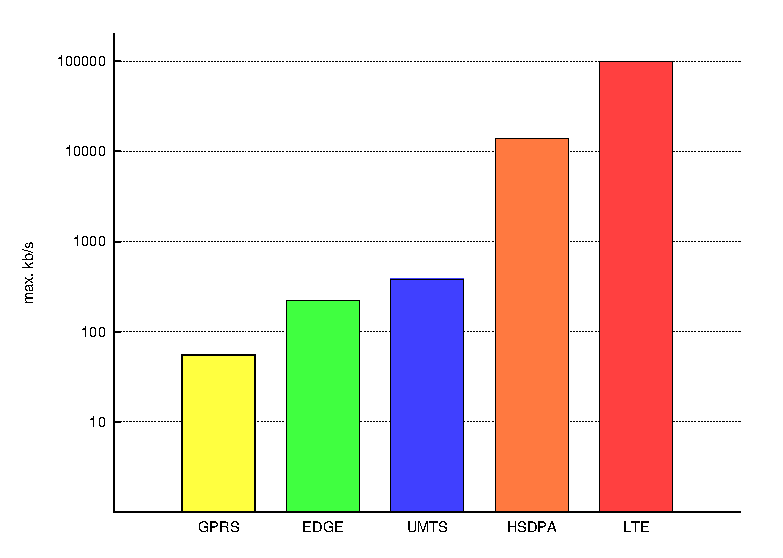
\includegraphics[width=\textwidth]{plot/datenraten}
     \caption{Vergleich der maximalen Datenraten von Mobilfunkstandards}
     \label{fig:datenraten}
 \end{figure}


 \subsection{Hersteller und Drittanbieter Lösungen} % {{{
 \label{sub:drittanbieter}

 % TODO: Quellen einfügen

 Durch die Anbindung des Internets an die Mobilfunknetze war es mit geeigneten Endgeräten
 möglich über Webdienste bekannte Instant Messaging-Protokolle wie \textit{XMPP} oder
 \textit{ICQ} zu nutzen. Der
 wirklich Durchbruch von alternativen Diensten zur SMS vollzog sich jedoch erst mit dem
 Aufkommen der sogenannten \glqq{}Smartphones\grqq{}. Mit diesen Geräten wurdes es zur Normalität,
 dass der Nutzer sich Software von Drittanbieter, sogenannte \glqq{}Apps\grqq{}, auf
 seinem Mobilfunkgerät installiert. Dadurch wurde wiederum zu erste Instant Messaging-Dienste,
 welche vom Desktop-Rechner bekannt waren, auf den Smartphones populär. Dazu zählen Apps für
 \textit{Skype} oder den \textit{Windows Live Messenger} aber auch Anwendungen, welche mehrer Protokolle
 unterstützen, wie \textit{Beejive} oder \textit{IM+}. Diese Dienste bieten allgemein die
 möglich kein eines Chats zwischen zwei oder mehreren Personen. Einige bieten zusätzlich noch die
 Möglichkeit der Audio- bzw. Videoübertragung. Zur Nutzung dieser Dienste ist jedoch eine
 Anmeldung bei jedem Dienst nötig und es ist auch nur möglich Personen zu erreichen, welche
 ebenfalls bei dem Dienst angemeldet sind.

 Ein wirklicher direkter Konkurrent der SMS wurde durch Herstellerlösungen wie
 Apples \textit{iMessage} oder BlackBerrys \textit{BlackBerry Messenger} geschaffen. Diese
 ermöglichen es Nutzer von Endgeräten dieser Hersteller untereinander kostenlose Nachrichten
 auszutauschen. Dazu ist oft keine aktive Anmeldung des Nutzers nötig, da sie eindeutig anhand
 der Endgeräte und ihrer Kundenidentifikation zugeordnet werden können. Der Nachteil der Dienste
 ist die Beschränkung auf Personen, welche ein Endgerät des selben Herstellers nutzen.

 Den weitaus größeren Erfolg versprechen Dienste von Drittanbietern, welche auf einer großen
 Anzahl von Plattformen verfügbar sind. Die bekanntesten und erfolgreichsten Anbieter
 sind hier \textit{WhatsApp} und \textit{kik}. Diese Dienste sind auf den größten
 Mobilenplatformen verfügbar, dazu zählen Android, iOS, Windows Mobile und BlackBerry OS. Der Nutzer wird über
 seine Mobilfunknummer identifiziert und muss sich nicht extra anmelden. Die Dienste sind meist mit
 nur geringen bis gar keinen Kosten verbunden und durch die weite Verbreitung stellen sie
 die größte Konkurrenz für die klassische SMS dar.
 % subsection Hersteller und Drittanbieter Lösungen }}}

 \subsection{Rich Communication Suite-enhanced} % {{{
 \label{sec:rcs-e}

  \textit{Rich Communication Suite-enhanced (RCS-e)} ist ein Industriestandard für die
  Kommunikation von mobilen Endgeräten. Er wird seit 2008 entwickelt und vorallem durch den
  Branchenverband \textit{GSM Association (GSMA)} vorangetrieben. Es werden verschiedene Standards der
  Organisationen \textit{3GPP}, \textit{OMA} und \textit{IETF} genutzt. Ein Überblick über die
  Komponenten der Version 5.0 des Standards ist in Abbildung \ref{fig:rcs-e-overview} zusehen.
  Die wichtigsten Bestandteile sind das Übermitteln von Nachrichten, Präsenzinformationen,
  Sprachtelefonie, Videoübertragung, Datenaustausch, Instant Messaging und Geolocation.

 \begin{figure}
     \centering
     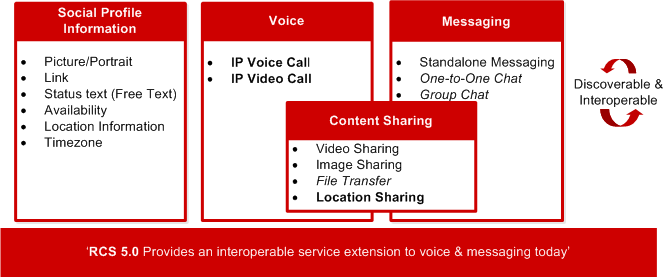
\includegraphics[width=\textwidth]{img/rcs-e-overview}
     \caption{Überblick der Komponenten des RCS-e 5.0 Standards \cite{rcs:spec}}
     \label{fig:rcs-e-overview}
 \end{figure}

  \subsubsection{Vermarktung} % {{{
  \label{ssub:vermarktung}

  Der Dienst soll wird unter dem Namen \textit{Joyn} als \glqq{}Nachfolger der
  SMS\grqq{} von den Mobilfunkanbieter vermarktet. Allerdings ist schon durch die pure Masse an
  Funktionen zu erkennen, dass der Dienst mehr umfasst als nur die
  Übertragung von Textnachrichten. Dieser neue Dienst soll von den wichtigensten
  Mobilplatformen unterstützt werden. Dazu sollen anfangs Apps angeboten werden aber im Laufe der
  Zeit soll eine direkte Integration in die mobilen Betriebssysteme erfolgen. Die Version 5.0
  des Standards wurde zum Zeitpunkt der GSMA \textit{Mobile World
      Congress (MWC)} 2012 in Spanien freigegeben. Gleichzeitig wurde auf der MWC eine
  funktionierende Implementation des Standards präsentiert. Anschließend startete Vodafone Spaninen
  eine Beta-Phase mit einer Android-App.

  In Deutschland wird Joyn seit September 2012 von Vodafone angeboten. Die Telekom plant mit dem
  1. Oktober 2012 als Starttermin. Von O2 ist noch kein Einführungstermin bekannt
  und E-Plus plant vorläufig überhaupt keine Einführung des Dienstes.

  % subsubsection Vermarktung }}}

  \subsubsection{Technik} % {{{
  \label{ssub:technik}

    Die grundlegende Architektur des RCS-e Standards bietet das \textit{IP Multimedia
        Subsystem (IMS)} der 3GPP. Darauf aufbauend wird das IETF \textit{Session Initiation
        Protocol (SIP)} zur Authentifizierung, Autorisierung, Registrierug und
    Abrechnung genutzt. Weitere OMA Standards werden zur Kommunikation zwischen den einzelnen
    Knoten des Systems genutzt. Das in der Abbildung \ref{fig:rcs-e-overview} aufgeführte
    \textit{Standalone Messaging} ist die eigentliche Weiterentwicklung der SMS/MMS. Daher wird im
    weiteren nur noch diese Funktion betrachtet.

    Die Funktion des \textit{Standalone Messaging} ermöglicht es Text- und Multimedianachrichten
    zu übertragen. Dabei ist es möglich Versand- und Displaymitteilungen zu erhalten. Außerdem wird
    eine sogenannter Multi-Device Unterstützung angeboten, dass heißt die Nachricht kann auf
    mehreren Endgeräten erhalten werden. Ein simples Beispiel ist dabei ein Nutzer, welcher ein
    Smartphone und ein Tablet besitzt, dieser könnte seine Nachrichten auf beiden Geräten
    empfangen, senden und anzeigen. Daraus leitet sich die Notwendigkeit eines Zentralen
    Nachrichtenspeichers zusätzlich zum Lokalen ab, da ansonsten das Verwalten aller
    Nachrichten, an mehreren Endgeräten nicht möglich wäre. Als Abwärtskompatibilität ist
    ein Austausch mit den klassischen SMS bzw. MMS Systemen möglich. Das heißt nutzer des
    Joyn-Dienstes können mit Nutzern kommunizieren, welche nicht Joyn nutzen.

    Die Nachrichten werden mittels OMA \textit{Converged IP Messaging (CPM)} übertragen. Dabei
    existieren zwei Modi, den \textit{Pager} und \textit{Large Mode}. Dabei hat der
    \textit{Pager Mode} eine Begrenzung von 1300 Byte. In Abbildung \ref{fig:rcs-e-pager} ist
    der Ablauf einer Nachrichtenübertragung mit Hilfe des CPM Pager Mode dargestellt. Dabei wird
    die SIP Methode \texttt{MESSAGE} genutzt um die Nachricht direkt zu übertragen. Da die
    Nachrichtengröße begrenzt ist, kann eine sichere und effiziente Vermittlung der Nachricht
    erreicht werden. Überschreitet die Nachricht, die 1300 Byte Begrenzung, wird der CPM
    Large Mode zur Übertragung genutzt. Der Ablauf einer solchen Übertragung ist in
    Abbildung \ref{fig:rcs-e-large} abgebildet. Um größere Nachrichten effizient zu übertragen
    wird dabei SIP nur zum Aufbau einer Sitzung genutzt. Die eigentlich Übertragung der Nachricht
    wird dann mit Hilfe des \textit{Message Session Relay Protocol (MSRP)} realisiert. Dies
    hat den Vorteil, dass das MSRP speziell für diese Anforderung ausgelegt ist und deshalb
    für größere Datenmengen besser geeignet ist als SIP.

    Die Anbindung an das klassische SMS-System ist in Abbildung \ref{fig:rcs-e-sms} skizziert.
    Dieser Fall tritt ein, wenn eine SMS an einen Joyn-Nutzer gesendet wird oder dieser eine
    \textit{Standalone Message} senden, deren Empfänger keine Joyn-Nutzer ist. Dabei
    entscheidet im letzteren Fall die Größe und Art der Nachricht, ob eine SMS oder MMS nötigt
    ist. Diese Überprüfung wird in der \textit{SMS Interworking Function (SMS-IWF)} durchgeführt.
    Ist die Nachricht als SMS zustellbar, wird sie in eine oder mehrere SMS umgewandelt und an das
    \textit{Short Message Service Centre (SMS-C)} weitergeleitet. Danach wird die Nachricht durch
    die bereits beschriebenen herkömmlichen Verfahren zugestellt.

 \begin{figure}
     \centering
     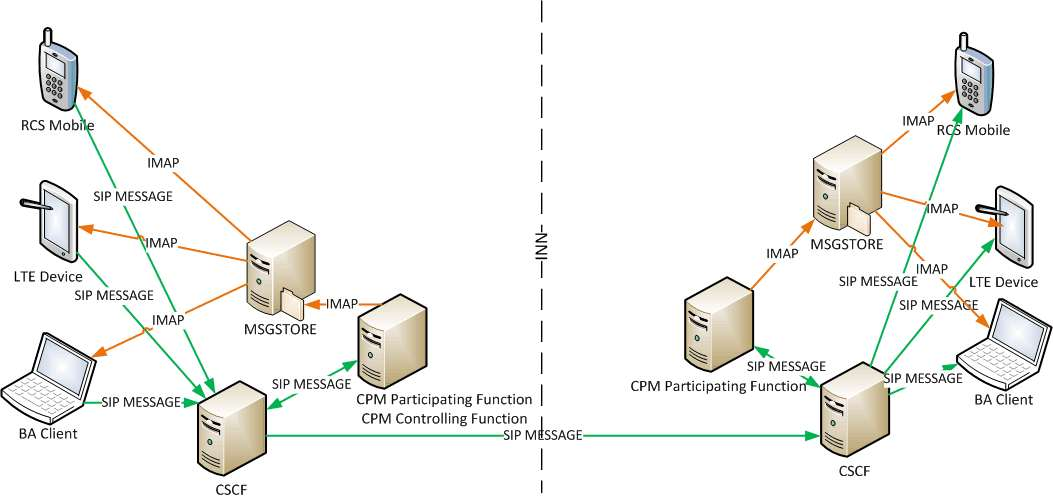
\includegraphics[width=\textwidth]{img/rcs-e-pager}
     \caption{RCS-e Nachrichtenübertragung im CPM Pager Mode \cite{rcs:spec}}
     \label{fig:rcs-e-pager}
 \end{figure}

 \begin{figure}
     \centering
     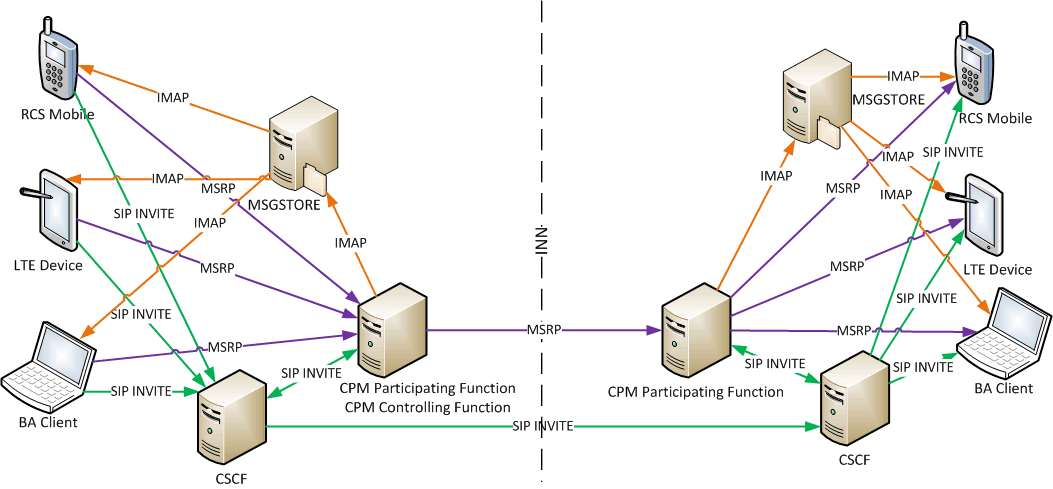
\includegraphics[width=\textwidth]{img/rcs-e-large}
     \caption{RCS-e Nachrichtenübertragung im CPM Large Mode \cite{rcs:spec}}
     \label{fig:rcs-e-large}
 \end{figure}

 \begin{figure}
     \centering
     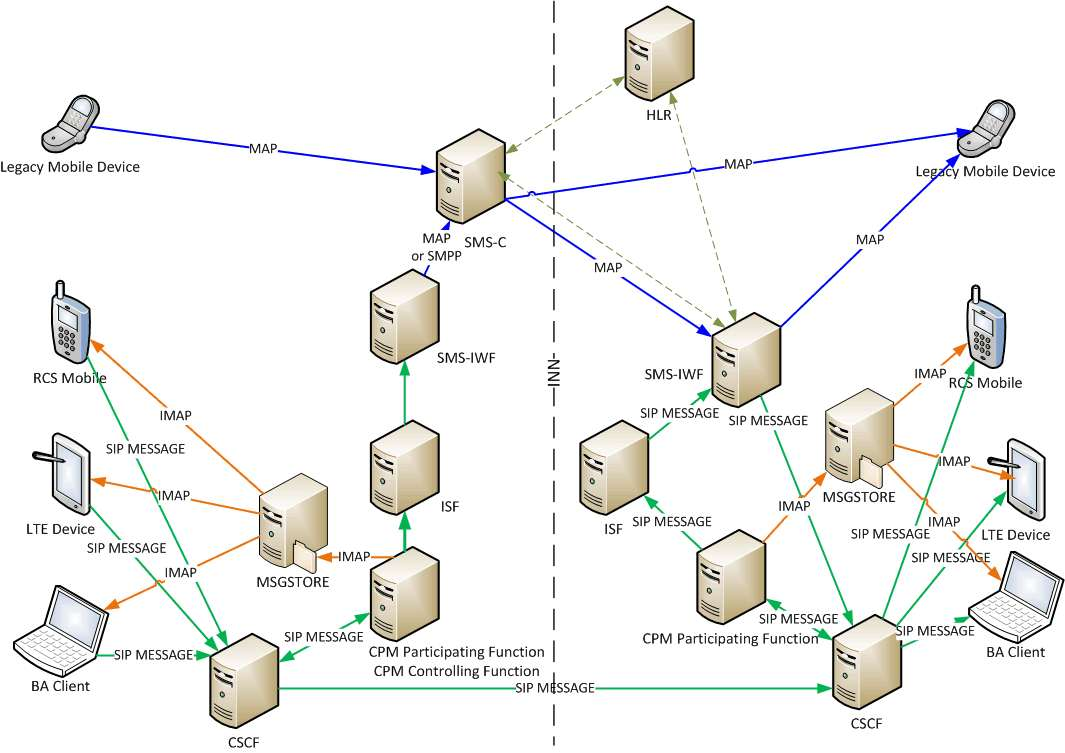
\includegraphics[width=\textwidth]{img/rcs-e-sms}
     \caption{RCS-e Nachrichtenübertragung mit SMS-Kompatibilität \cite{rcs:spec}}
     \label{fig:rcs-e-sms}
 \end{figure}

  % subsubsection Technik }}}

 % subsection Rich Communication Suite-enhanced }}}

 \subsection{Vergleich} % {{{
 \label{sub:vergleich}

    Der RCS-e Standard ist eine positive Entwicklung zur Vereinheitlichung der
    Multimedialen-Kommunikation. Der Standard enthält alle wichtigen Funktionen moderner
    Kommunikation und wird von den größten Mobilfunkunternehmen unterstützt. Allerdings
    haben die beschriebenen Alternative zur Zeit noch die größere Verbreitung. Dies liegt
    zuerst daran, dass der Joyn-Dienst gerade erste mit den ersten Anbietern startet. Die
    weitere Entwicklung wird vor allem von der Umsetzung durch die Mobilfunkanbieter
    abhängen.

    Im Vergleich haben die Hersteller-Dienste den Vorteil, dass sie immer direkt im Betriebssystem
    verankert sind, kostenlos und ohne Anmeldung funktionieren und jeder Nutzer die gleich
    Funktionalität besitzt. Allerdings sind sie nur auf die herstellereigenen
    Endgeräte begrenzt. Die Drittanbierter-Apps sind hingegen auf den meiseten Plattformen
    verfügbar und haben ebenfalls einen einheitlichen Funktionsumfang. Allerdings muss dazu der
    Nutzer seine Daten an einen zusätzliche Anbieter preisgeben. Der Joyn-Dienst soll zwar auch
    plattformübergreifend verfügbar werden, allerdings handelt es sich um einen offenen Standard.
    Dabei entscheidet der Mobilfunkanbieter, welcher Funktionen er umsetzt und anbietet. Hierbei
    wäre es möglich alle interessanten Kommunikationsfunktionen zu vereinen und eine Verlässlichkeit
    ähnlich der SMS anzubieten.

 % subsection Vergleich }}}

% section SMS über Datennetze }}}

\section{Fazit} % {{{
\label{sec:fazit}

Die Einführung der RCS-e Dienste ist zwar noch nicht vollständig abgeschloßen, jedoch
kann man davon ausgehen, dass der Dienst nicht ohne weiteres die SMS verdrängen wird. Die
Nachteile der SMS, mit ihrer Begrenztheit, sind klar erkennbar, allerdings hat sie sich innerhalb
der Jahre zu einem stabilen, zuverlässigen System entwickelt. Jedes Mobilfunkgerät kann
heutzutage SMS senden und empfangen. Trotz der fragwürdigen Preispolitik der Mobilfunkanbieter,
wird die SMS immer der kleinste Nenner sein, welcher von allen Teilnehmer genutzt werden kann.
Vor allem solange keine komplette Abdeckung mit schnelleren Datennetze erreicht ist, wird die
SMS nicht abschaffbar sein. Ist jedoch für den Nutzer ein Datennetz verfügbar so sind die
Vorteile der neuen Nachrichtendienste eindeutig. Besonders die rasante Verbreitung von
Smartphones und der große Erfolg von Diensten wie \textit{WhatsApp} zeigen, dass
Alternative nötig sind und auch angenommen werden. Die Einführung von RCS-e Diensten könnte in
diesem Zusammenhang eine wichtige Rolle spielen. Da dieser Standard alle wichtigen Dienste
abdeckt, welche bis jetzt von keinem Angeboten alleine angeboten wird, könnte er eine große
Verbreitung erreichen. Da zu diesem Zeitpunkt keine Aussage über die Umsetzung des Standards
durch die Mobilfunkanbieter getroffen werden kann, er geben sich vorallem zwei Punkte, welche über
den Erfolg von Joyn entscheiden werden. Der eine Faktor ist die Preispolitik der
Mobilfunkanbieter. Bei SMS existierte ein Monopol und dementsprechend war die Preisgestaltung. Wie
in Abschnitt \ref{sec:datennetze} gezeigt ist Joyn bei seiner Einführung nicht Konkurrenzlos.
Viele Alternative sind kostenlos oder haben sehr geringe Kosten, welche nicht vergleichbar mit
normalen Mobilfunktarifen sind. Allerdings hat Joyn den Vorteil, dass es ein Dienst von den
Mobilfunkbetreibern ist. Das heißt es besteht die Möglichkeit, das es wieder zu einer
Selbstverständlichkeit wie SMS wird. Also das jedes Endgerät Joyn unterstützt ohne das der Nutzer
dies konfigurieren muss oder groß über die Verwendung nachdenken muss. Leider spricht gegen diese
Entwicklung der Verlauf der Einführung des Diensts. Es gibt keine einheitliche Einführung und auch
die geplanten Termine konnte nicht eingehalten werden. Hinzukommt eine schlechte Vermarktung bis zum
jetzigen Zeitpunkt ist der Dienst und seine Funktionen kaum bekannt bei den Nutzern. Allerdings
könnten diese Nachteile in ein paar Jahren vergessen sein. Die aktuelle Fluktuation von Endgeräten
ist nicht mehr vergleichbar mit den Anfängen der mobilen Kommunikation. Sollte es die
Mobilfunkbetreiber schaffen Joyn so in den Endgeräten zu verankern, dass es bereits bei der
Inbetriebnahme vorhanden und konfiguriert ist, so könnte sich mit einer angemessenen Preisstruktur
eine ähnlich alltäglich Nutze einstellen, welche mit der SMS vergleichbar ist.

% section Fazit }}}

\clearpage
\bibliography{cites}

\end{document}
